\documentclass[12pt,english]{article}

\usepackage{amsmath,amssymb,amsthm,epsfig,lineno,rotfloat,psfrag,natbib,caption,setspace,url,bm,geometry}
\usepackage{ecology}
%\usepackage{nameref,hyperref}


\geometry{verbose,letterpaper,tmargin=2.54cm,bmargin=2.54cm,lmargin=2.54cm,rmargin=2.54cm}

%\setlength{\evensidemargin}{0in} \setlength{\oddsidemargin}{0in}
%\setlength{\topmargin}{-0.65in} \setlength{\textwidth}{6.5in}
%\setlength{\textheight}{9.5in} \setlength{\topskip}{0in}
%\setlength{\headheight}{0in}

\bibpunct{(}{)}{,}{a}{}{;}

%\renewcommand{\includegraphics}[2][]{}

\bibliographystyle{ecology}
\raggedbottom


\captionsetup[table]{margin=0pt,font=small,labelfont={sc},justification=justified,labelsep=period}
\captionsetup[figure]{margin=0pt,font=small,labelfont={sc},justification=justified,labelsep=period,name=Fig}



\begin{document}
\begin{spacing}{1.9}


\begin{center}
A guide to Bayesian model checking for ecologists
\bigskip\\
\normalsize
{\sc Paul B. Conn$^{1,}$\footnotemark[5], Mevin B. Hooten$^{2,3,4}$, and
Devin S. Johnson$^1$ }\smallskip\\
$^1${\em National Marine Mammal Laboratory, NOAA, National Marine Fisheries Service,
Alaska Fisheries Science Center, 7600 Sand Point Way NE, Seattle,
WA 98115 USA }\\ \medskip
$^2${\em U.S. Geological Survey, Colorado Cooperative Fish and Wildlife Research Unit, Colorado State University, Fort Collins, CO 80523 USA }\\ \medskip
$^3${\em Department of Fish, Wildlife, and Conservation Biology, Colorado State University, Fort Collins, CO 80523 USA }\\ \medskip
$^4${\em Department of Statistics, Colorado State University, Fort Collins, CO 80523 USA }\\ \medskip
\end{center}
\footnotetext[5]{Email: paul.conn@noaa.gov}


\raggedright \setlength{\parindent}{0.3in}
%\renewcommand{\baselinestretch}{1.8}\normalsize
\clubpenalty=0

\linenumbers

{\em Abstract.\ }  Checking that models adequately represent data is
an essential component of applied statistical inference.  Ecologists
increasingly use hierarchical Bayesian statistical models in their
research.  The appeal of this modeling paradigm is undeniable, as
researchers can build and fit models that embody complex ecological
processes while simultaneously controlling for potential biases
arising from sampling artifacts. However, ecologists tend to be less
focused on checking model assumptions and assessing potential
lack-of-fit when applying Bayesian methods than when they applying
more traditional modes of inference such as maximum likelihood.  There
are also multiple ways of assessing goodness-of-fit for Bayesian
models, each of which has strengths and weaknesses.  For instance, in
ecological applications, the posterior predictive p-value is probably
the most widely used approach for assessing lack of fit in Bayesian
models. Such p-values are relatively easy to compute, but they are
well known to be conservative, producing p-values biased toward 0.5.
Alternatively, lesser known approaches to model checking, such as
prior predictive checks, cross-validation probability integral
transforms, and pivot discrepancy measures may produce more accurate
characterizations of goodness-of-fit but are not as well known to
ecologists.  In addition, a suite of visual and targeted diagnostics
can be used to examine violations of different model assumptions and
lack-of-fit at different levels of the modeling hierarchy, and to
check for residual temporal or spatial autocorrelation.  In this
review, we synthesize existing literature in order to guide ecologists
to the many available options for Bayesian model checking.  We
illustrate methods and procedures with several ecological case
studies, including i) explaining variation in simulated
spatio-temporal count data, and (ii) modeling survival and residence
times of fur seal mothers on a rookery, and (iii) using N-mixture
models to model sea otters.  We find that commonly used procedures based on posterior predictive p-values have high power to detect extreme model inadequacy, but low power to detect more subtle cases of lack of fit.  Tests based on cross-validation and pivot discrepancy measures (including the ``sampled predictive p-value") appear to be much better suited to this task and to have better overall statistical performance. We conclude that model checking is an essential component of scientific discovery and learning that should accompany most Bayesian analyses presented in the literature.


{\em Bayesian p-value, count data, goodness-of-fit diagnostic check, hierarchical model, model checking, N-mixture model, pivot discrepancy, posterior predictive check, probability interval transform, sampled predictive p-value, spatio-temporal model}



\def\VAR{{\rm Var}\,}
\def\COV{{\rm Cov}\,}
\def\Prob{{\rm P}\,}
\def\bfx{{\bf x}}
\def\bfX{{\bf X}}
\def\bfY{{\bf Y}\,}
\def\bfy{{\bf y}}
\def\bfZ{{\bf Z}\,}
\def\bftheta{\boldsymbol{\theta}}
\def\bfeta{\boldsymbol{\eta}}
\def\bfOmega{\boldsymbol{\Omega}}
\def\bfbeta{\boldsymbol{\beta}}
\def\bfSigma{\boldsymbol{\Sigma}}
\def\bfmu{\boldsymbol{\mu}}
\def\bfnu{\boldsymbol{\nu}}
\def\bfepsilon{\boldsymbol{\epsilon}}
\def\R2{\rm I\!R^2}


\section{Introduction}

Ecologists increasingly use Bayesian methods to analyze complex hierarchical models for natural systems \citep{HobbsHooten2015}.  There are clear advantages of adopting a Bayesian mode of inference, as one can entertain models that were previously intractable using common modes of statistical inference (e.g., maximum likelihood). Ecologists use Bayesian inference to fit rich classes of models to their datasets, allowing them to separate measurement error from process error, and to model features such as temporal or spatial autocorrelation, individual level random effects, and hidden states \citep{LinkEtAl2002,ClarkBjornstad2004,CressieEtAl2009}. Applying Bayesian calculus also results in posterior probability distributions for parameters of interest; used together with posterior model probabilities, these can provide the basis for mathematically coherent decision and risk analyses \citep{LinkBarker2006,Berger2013,WilliamsHootenInPress}.

Ultimately, the reliability of inference from a fitted model (Bayesian or otherwise) depends on how well the model approximates reality.  There are multiple ways of assessing a model's performance in representing the system being studied. A first step is often to examine diagnostics that compare observed data to model output to pinpoint if and where any systematic differences occur. This process, which we term \textit{model checking}, is a critical part of statistical inference, as it helps diagnose assumption violations and illuminate places where a model might be amended to more faithfully represent gathered data. Following this step, one might proceed to compare the performance of alternative models embodying different hypotheses using any number of model comparison or out-of-sample predictive performance metrics \citep[see][for a review]{HootenHobbs2015} to gauge the support for alternative hypotheses or optimize predictive ability (Fig. \ref{fig:decision}).  Note that scientific inference can still proceed if models do not fit the data well, but conclusions need to be tempered; one approach in such situations is to estimate a variance inflation factor to adjust precision levels downward \citep[e.g.,][]{CoxSnell1989,McCullaghNelder1989}.

Non-Bayesian statistical software often include a suite of goodness-of-fit diagnostics that examine different types of lack-of-fit (Table \ref{tab:lof}).  For instance, when fitting generalized linear \citep{McCullaghNelder1989} or additive \citep{Wood2006} models in the R programming environment \citep{RTeam2015}, one can easily access diagnostics such as quantile-quantile, residual, and leverage plots.  These diagnostics allow one to assess the reasonability of the assumed probability model, to examine whether there is evidence of heteroskedasticity, and to pinpoint outliers.  Likewise, in capture-recapture analysis, there are established procedures for assessing overall fit as well as departures from specific model assumptions which are codified in user-friendly software such as U-CARE \citep{ChoquetEtAl2009}.  Results of such goodness-of-fit tests are routinely reported when publishing analyses in the ecological literature.

The implicit requirement that one conduct model checking exercises is not often adhered to when reporting results of Bayesian analyses in the ecological literature.  For instance, a search of recent volumes of Ecology indicated that only 25\% of articles employing Bayesian analysis on real datasets reported any model checking or goodness-of-fit testing (Fig. \ref{fig:WOS}).  There are several reasons why Bayesian model checking is uncommon.  First, it likely has to do with momentum; the lack of precedent in ecological literature may lead some authors looking for templates on how to publish Bayesian analyses to conclude that model checking is unnecessary.  Second, when researchers seek to publish new statistical methods, applications may be presented more as proof-of-concept exhibits than as definitive analyses that can stand up to scrutiny on their own. In such studies, topics like goodness-of-fit and model checking are often reserved for future research, presumably in journals with less impact.  Third, all of the articles we examined did a commendable job in reporting convergence diagnostics to support their contention that Markov chains from MCMC output had reached their stationary distribution.  Perhaps there is a mistaken belief among authors and reviewers that convergence to a stationary distribution, combined with a lack of prior sensitivity, implies that a model fits the data?  Finally, it may just be that those publishing Bayesian analyses in ecological literature ``. . . like artists, have the bad habit of falling in love with their models" (to borrow a quote attributed to G.E.P. Box and referenced by \citet{LinkBarker2010} with regard to model checking).  However, models can be poor at returning our affection; indeed this monograph can be viewed as a partial atonement for unrequited love.

If we accept the premise that Bayesian models in ecology should be routinely checked for compatibility with data, a logical next question is how best to conduct such checks.  Unfortunately, there is no single best answer.  Most texts in ecology \citep[e.g.,][]{KingEtAl2009,LinkBarker2010,KerySchaub2012} focus on posterior predictive checks, as pioneered by \citet{Guttman1967}, Rubin (\citeyear{Rubin1981,Rubin1984}), and \citet{GelmanEtAl1996} (among others).  These procedures are also the main focus of popular Bayesian analysis texts \citep[e.g.,][]{CressieWikle2011,GelmanEtAl2014} and are based on the intuitive notion that data simulated from the posterior distribution should be similar to the data one is analyzing.  However, ``Bayesian p-values" generated from these tests tend to be conservative (biased toward 0.5) because the data are used twice \citep[once to fit the model and once to test the model;][]{BayarriBerger2000,RobinsEtAl2000}.  Depending on the data, the conservatism of Bayesian p-values can be considerable \citep{Zhang2014} and can be accompanied by low power to detect lack-of-fit \citep{YuanJohnson2012,Zhang2014}. By contrast, other approaches less familiar to ecologists (such as prior predictive checks, sampled posterior p-values, cross-validated probability integral transforms, and pivot discrepancy measures) may produce more accurate characterizations of model fit.

In this monograph, we have collated relevant statistical literature with the goal of providing ecologists with a practical guide to Bayesian model checking.  We start by defining a consistent notation that we use throughout the paper. Next, we work to compile a bestiary of Bayesian model checking procedures, providing positives and negatives associated with each approach.  We illustrate Bayesian model checking using several simulation studies (including spatial regression and ...), as well as a case study involving capture-recapture sampling of adult female fur seals (\textit{Callorhinus ursinus}) on a rookery in Alaska, U.S.A..  We conclude with several recommendations on how model checking results should be presented in the ecological literature.



\section{Background and notation}

Before describing specific model checking procedures, we first establish common notation.  Bayesian inference seeks to describe the posterior distribution, $[\boldsymbol{\theta} | {\bf y}]$, of model parameters, $\boldsymbol{\theta}$, given data, \textbf{y}.  Throughout the paper, we use bold lowercase symbols to denote vectors.  Matrices are represented with bold, uppercase symbols, while roman (unbolded) characters are used for scalars.  The bracket notation `$[ \hdots ]$' denotes a probability distribution or mass function, and a bracket with a vertical bar `$|$' denotes that it is a conditional probability distribution.

The posterior distribution is often written as
\begin{eqnarray}
  [\boldsymbol{\theta} | \textbf{y}] & = & \frac{[\textbf{y} | \boldsymbol{\theta}] [\boldsymbol{\theta}]}{[\textbf{y}]},
\end{eqnarray}
where $[\textbf{y}|\boldsymbol{\theta}]$ is the assumed probability model for the data, given parameters (i.e., the likelihood), $[\boldsymbol{\theta}]$ denotes the joint prior distribution for parameters, and $[\textbf{y}]$ is the marginal distribution of the data.  In Bayesian computation, the denominator $[\textbf{y}]$ is frequently ignored because it is a fixed constant that does not affect inference \citep[although it is needed when computing Bayes factors for model comparison and averaging;][]{LinkBarker2006}.
The exact mechanics of Bayesian inference are well reviewed elsewhere \citep[e.g.,][]{KingEtAl2009,LinkBarker2010,HobbsHooten2015}, and we do not attempt to provide a detailed description here.  For the remainder of this treatment, we assume that the reader has familiarity with the basics of Bayesian inference, including Markov chain Monte Carlo (MCMC) as a versatile tool for sampling from $[\boldsymbol{\theta}|\textbf{y}]$.

In describing different model checking procedures, we often refer to data simulated under an assumed model.  We use $\textbf{y}_i^{rep}$ to denote a single, simulated dataset under the model that is being checked.  In some situations, we may indicate that the dataset was simulated using a specific parameter vector, $\boldsymbol{\theta}_i$; in this case, denote the simulated dataset as $\textbf{y}_i^{rep}|\boldsymbol{\theta}_i$.  We use the notation $T(\textbf{y},\boldsymbol{\theta})$ to denote a discrepancy function that is dependent upon data and possibly the parameters $\boldsymbol{\theta}$.  For instance, we might compare the  discrepancy $T(\textbf{y},\boldsymbol{\theta})$ calculated with observed data to a distribution obtained by applying $T(\textbf{y}^{rep},\boldsymbol{\theta})$ to multiple replicated data sets.  Examples of candidate discrepancy functions are provided in Table \ref{tab:discrepancy}.

\section{Model checking procedures}

Our goal in this section is to review relevant Bayesian model checking procedures for typical models in ecology, with the requirement that such procedures be accessible to statistics-savvy ecologists.  As such, we omit several approaches that have good statistical properties but have been criticized \citep[e.g.,][]{Johnson2007b,Zhang2014} as too computationally intensive, conceptually difficult, or problem-specific to be of relevant use in common applications.  For instance, we omit consideration of double sampling methods that may increase the computational burden of a Bayesian analysis by an order of magnitude \citep{Johnson2007b}, including  ``partial posterior" and ``conditional predictive" p-values \citep[see e.g.,][]{BayarriBerger1999,RobinsEtAl2000,BayarriCastellanos2007}.

\subsection{Prior predictive checks}

\citet{Box1980} argued that the hypothetico-deductive process of scientific learning can be embodied through successive rounds of model formulation and testing. According to his view, models are built to represent current theory and an investigator's knowledge of the system under study; data are then collected to evaluate how well the existing theory (i.e., model) matches up with reality.  If necessary, the model under consideration can be amended, and the process repeats itself.

From a Bayesian standpoint, such successive rounds of \textit{estimation} and \textit{criticism} can be embodied through posterior inference and model checking, respectively \citep{Box1980}.
If one views a model, complete with all its set of assumptions and prior beliefs, as a working model of reality, then data simulated under a model should look similar to data gathered in the real world.  This notion can be formalized through a prior predictive check, where replicate data $\bfy^{rep}$ are simulated via
\begin{eqnarray}
   \label{eq:prior}
   \bftheta^{rep} & \sim & [\bftheta] \\
   \bfy^{rep} & \sim & [\bfy|\bftheta^{rep}] \nonumber
\end{eqnarray}
and then compared to observed data $\bfy$ via a discrepancy function (Appendix A, Alg. 1).

When the prior distribution(s) $[\bftheta]$ are proper statistical distributions, p-values from prior predictive checks are uniformly distributed under the null model and have properly stated frequentist properties.  The main problem with this approach is that the models being considered need to have considerable historical investment and proper prior distributions informed by expert opinion or data from previous studies.  In our experience, when Bayesian inference is employed in ecological applications, this is not often the case.  Still, prior predictive checks may be useful for hierarchical models that serve as an embodiment of current theory about a study system (e.g., population or ecosystem dynamics models).  Alternatively, a subset of data (test data) can be withheld when fitting a model, and the posterior distribution $[\bftheta|\bfy]$ can be substituted for $[\bftheta]$ in Eq. \ref{eq:prior}.  If used in this manner, prior predictive checks can be viewed as a form of cross validation, a subject we shall examine in a later subsection (see \textit{Cross-validation tests}).

Prior predictive checks appear to have found little use in applied Bayesian analysis \citep[but see][]{DeyEtAl1998}, at least in the original form proposed by \citet{Box1980}. However, they are important as historical precursor to modern day approaches to Bayesian model checking. Further, several researchers have recently used discrepancy measures calculated on prior predictive data sets to help calibrate posterior predictive \citep[e.g.,][]{HjortEtAl2006} or joint pivot discrepancy \citep{Johnson2007} p-values so that they have a uniform null distribution.  These calibration exercises are not conceptually difficult, but do have a high computational burden \citep{YuanJohnson2012}. The properties (e.g., type I error probabilities, power) of p-values produced with these methods also depend critically on the similarity of the real world data-generating process with the prior distributions used for calibration \citep{Zhang2014}.

\subsection{Posterior predictive checks}

Posterior predictive checks are the dominant form of Bayesian model checking advanced in statistical texts read by ecologists \citep[e.g.,][]{KingEtAl2009,LinkBarker2010,KerySchaub2012,GelmanEtAl2014}. Although sample size was small ($n=25$), our survey of recent \textit{Ecology} volumes indicated that posterior predictive checks are also the dominant form of Bayesian model checking being reported in ecological literature (if any checking is reported at all; Fig. \ref{fig:WOS}).  Posterior predictive checks are based on the intuition that data simulated under a fitted model should be comparable to the real world data the model was fitted to. If observed data differ from simulated data in a systematic fashion (e.g., excess zeros, increased skew, lower kurtosis), it is good indication that model assumptions are not being met.

Posterior predictive checks can be used to look at differences between observed and simulated data graphically, or can be used to calculate ``Bayesian p-values" (Appendix A, Alg. 2).  Bayesian p-values necessarily involve application of a discrepancy function, $T(\textbf{y},\boldsymbol{\theta})$, for comparing observed and simulated data.  There are several omnibus discrepancy measures that can be employed to examine overall lack-of-fit, and targeted discrepancy measures can be used to look for specific data features that systematically differ between simulated and observed data (Table \ref{tab:discrepancy}).

Posterior predictive checks are straightforward to implement.  Unfortunately, Bayesian p-values based on these checks tend to be conservative in the sense that the distribution of p-values calculated under a null model (i.e., when the data generating model and estimation model are the same) tends to be dome shaped instead of the uniform distribution expected of frequentist p-values \citep{RobinsEtAl2000}. This feature arises because data are used twice: once to approximate the posterior distribution and to simulate the reference distribution for the discrepancy measure, and a second time to calculate the tail probability  \citep{BayarriBerger2000}.  As such, the power of posterior predictive Bayesian p-values to detect significant differences in the discrepancy measure is low.  Evidently, the degree of conservatism can vary across data, models, and discrepancy functions, making it difficult to interpret or compare Bayesian p-values across models. In a simulation study with two different model types, \citet{Zhang2014} found that posterior predictive p-values almost never rejected a model, even when the model used to fit the data differed considerably from the model used to generate it.

Another possible criticism of posterior predictive checks is that they rely solely on properties of simulated and observed data.  Given that a lack of fit is observed, it may be difficult to diagnose where misspecification is occurring within the modeling hierarchy (e.g., poorly specified priors, errant mean structure, underdispersed error distribution).  Further, a poorly specified mean structure may still result in reasonable fit of the model if the model is made sufficiently flexible through inclusion of random effects.

These cautions do not imply that posterior predictive checks are completely devoid of value.  Indeed, given that tests are conservative, small (e.g., $<0.05$) or very large (e.g., $>0.95$) p-values strongly suggest lack-of-fit.  Further, graphical displays (see \textit{Graphical techniques}) and targeted discrepancies (Table \ref{tab:discrepancy}) may help pinpoint common assumption violations (e.g., lack of independence, zero inflation, overdispersion).  However, it is often less clear how to interpret p-values and discrepancies that indicate no (or little) lack-of-fit. P-values close to 0.15 or 0.25 are especially problematic.  In these cases, it seems necessary to conduct simulation-based exercises to determine the range of p-values that should be regarded as extreme, and to possibly calibrate the observed p-value with those obtained in simulation exercises \citep[e.g.,][]{DeyEtAl1998,HjortEtAl2006}.

Some practical suggestions may help to reduce the degree of conservatism of posterior predictive p-values.  \citet{LunnEtAl2013} suggest that the level of conservatism depends on the discrepancy function used; discrepancy functions that are solely a function of simulated and observed data (e.g., proportion of zeros, distribution of quantiles) may be less conservative than those that also depend on model parameters (e.g., summed Pearson residuals).  Similarly, \citet{MarshallSpiegelhalter2003} suggest reducing the impact of the double use of data by iteratively resimulating random effects when generating posterior predictions for each data point, a procedure they term a ``mixed predictive check" (also called ``ghosting").  For an example of this latter approach, see \textit{Spatial models for count data}.

\subsection{Sampled posterior p-values}

Posterior predictive checks involve cyclically drawing parameter values from the posterior distribution (i.e., $\bftheta_i \sim [\bftheta| \bfy]$) and then generating a replicate dataset for each $i$, $\bfy_i^{rep} \sim [\bfy | \bftheta_i]$, to compute the reference distribution for a discrepancy test statistic \citep[][; Appendix A, Alg. 2]{GelmanEtAl2004}.  Alternatively, one can simulate a single parameter vector from the posterior, $\tilde{\bftheta} \sim [\bftheta| \bfy]$, and then generate replicate datasets conditional on this parameter vector alone (i.e., $\bfy_i^{rep} \sim [\bfy | \tilde{\bftheta}]$), otherwise calculating the p-value in the same manner.  This choice may seem strange because the resulting p-value can vary depending upon the posterior sample, $\tilde{\bftheta}$, but a variety of theoretical arguments \citep[e.g.,][]{Johnson2004,Johnson2007,YuanJohnson2012,Gosselin2011} and several simulation studies \citep[e.g.,][]{Gosselin2011,Zhang2014} suggest that it may be a preferable choice, both in terms of Type I error control and power to detect lack-of-fit.  In fact, sampled posterior p-values are guaranteed to at least have an asymptotic uniform distribution under the null \citep[i.e., when the model fit to the data is the ``true" model][]{Gosselin2011}.  Sampled posterior p-values can also be calculated using pivotal discrepancy measures, reducing computational burden (i.e., eliminating the requirement that replicate datasets be generated). We describe an example of this approach in \textit{Spatial models for count data}.

\subsection{Pivotal discrepancy measures (PDMs)}

In addition to overstated power to detect model lack-of-fit, posterior predictive p-values are limited to examining systematic differences between observed data and data simulated under a hypothesized model.  As such, there is little ability to examine lack-of-fit at higher levels of modeling hierarchy.  One approach to conducting goodness-of-fit at multiple levels of the model is to use discrepancy functions based on pivotal quantities \citep{Johnson2004,YuanJohnson2012}.  Pivotal quantities are random variables that can be functions of data, parameters, or both, that have known probability distributions that are independent of parameters \citep[see e.g.,][section 9.2.2]{CasellaBerger1990}.  For instance, if
\begin{eqnarray*}
  y & \sim & \mathcal{N}(\mu,\sigma^2)
\end{eqnarray*}
then $z = \frac{y-\mu}{\sigma}$ has a standard $f=\mathcal{N}(0,1)$ distribution. Thus, $z$ is a pivotal quantity in that it has a known distribution independent of $\mu$ or $\sigma$.

This suggests a potential strategy for assessing goodness-of-fit; for instance, in a Bayesian regression model
\begin{eqnarray}
  \label{eq:reg}
  {\bf y} & \sim & \mathcal{N}(\textbf{X} \boldsymbol{\beta},\sigma^2 \textbf{I}),
\end{eqnarray}
where $\textbf{X}$ represents a design matrix, $\boldsymbol{\beta}$ is a vector of regression coefficients, and $\textbf{I}$ is an identity matrix, we might keep track of
\begin{eqnarray}
  \label{eq:resid}
  z_{ij} & = & \frac{y_i - \textbf{x}_i^\prime \boldsymbol{\beta}_j}{\sigma_j}
\end{eqnarray}
for each of $j \in {1, 2, \hdots, n}$ samples from the posterior distribution (i.e., drawing each $(\boldsymbol{\beta}_j, \sigma_j)$ pair from  $[\boldsymbol{\theta}|{\bf y}]$).  Systematic departures of $z_{ij}$ from the theoretical $\mathcal{N}(0,1)$ distribution can point to model misspecification.  Although we have focused on the data model in Eq. \ref{eq:reg}, note that the same approach could be used at higher levels of the modeling hierarchy.

The advantage of using PDMs is that the reference distribution is known and does not necessarily involve simulation of replicated datasets, $\bfy^{rep}$.  However, in practice, there are several difficulties with using pivotal quantities as discrepancy measures in Bayesian model checking.  First, as with the sampled predictive p-value, p-values using PDMs are only guaranteed to be uniform under the null if calculated with respect to a single posterior parameter draw, $\tilde{\bftheta} \sim [\bftheta | \bfy]$.  The joint distribution of PDMs calculated across $i \in 1,2,\hdots,n$ samples from the posterior distribution are not independent because they depend on the same observed data, $\textbf{y}$ \citep{Johnson2004}.  As with the Bayesian p-value calculated using a posterior predictive check, this latter problem can result in p-values that are conservative.  \citet{YuanJohnson2012} suggest comparing histograms of a pivotal discrepancy function $T(\textbf{y},\boldsymbol{\theta}_i)$ to its theoretical distribution, $f$, to diagnose obvious examples of model misspecification.  If an omnibus Bayesian p-value is desired, a test can be implemented by appealing to limiting distributions of order statistics \citep{Johnson2004}, but these tests are conservative and have low power to detect lack of fit.

A second problem is that, to apply these techniques, one must first define a pivotal quantity and ascertain its reference distribution. Normality assessment is relatively straightforward using standardized residuals (e.g., Eq. \ref{eq:resid}), but pivotal quantities are not necessarily available for other distributions (e.g., Poisson).  However, \citet{YuanJohnson2012}, building upon work of \citet{Johnson2004} proposed an algorithm based on cumulative distribution functions (CDFs) that can apply to any distribution, and at any level of a hierarchical model (Appendix A, Alg. 3).  For continuous distributions, this algorithm works by defining a quantity $w_{ij} = g(y_{ij},\boldsymbol{\theta})$ (this can simply be $w_{ij}=y_{ij}$) with a known CDF, $F$.  Then, according to the probability integral transformation, $F({\bf w})$ should be uniformly distributed if the the modeled distribution function is appropriate.  Similarly, for discrete distributions, we can apply a randomization scheme \citep{Smith1985,YuanJohnson2012} to transform discrete variables into continuously distributed uniform variates.  For example, when $y_{ij}$ has integer valued support, we can define
\begin{eqnarray*}
  w_{ij} & = & F(y_{ij}-1|\boldsymbol{\theta}) + u_{ij} f(y_{ij}|\boldsymbol{\theta}),
\end{eqnarray*}
where $u_{ij}$ is a continuosly uniform random deviate on (0,1) and $F()$ and $f()$ are the cumulative mass and probability mass functions associated with $[{\bf y} | \boldsymbol{\theta}]$, respectively.  In this case, $w_{ij}$ will be uniformly and continuously distributed on (0,1) if the assumed distribution is reasonable; deviation from uniformity can point to model misspecification.

We have written the PDM algorithm in terms of the data distribution $[{\bf y} | \boldsymbol{\theta}]$ (Appendix A), but the algorithm can be applied (without loss of generality) to any level of a hierarchical model. Further, the algorithm can be applied separately to different categories of mean response (e.g., low, medium, or high levels of predicted responses). These advantages are extremely appealing in that one can more thoroughly test distributional assumptions and look for places where lack-of-fit may be occurring, something that can be difficult to do with posterior predictive checks.  We apply this algorithm in \textit{Examples} and provide R code for applying this approach to generic MCMC data in the R package \texttt{HierarchicalGOF} accompanying this paper (see \textit{Software} for more information).



\subsection{Cross-validation tests}

Cross-validation consists of leaving out one or more data points, running an analysis, and seeing how model predictions match up with actual observations.  This process is often repeated sequentially for different partitions of the data.  It is most often used to examine the relative predictive performance of different models \citep[i.e., for model selection; see e.g.][]{ArlotCelisse2010}.  However, it also possible to use cross-validation techniques to examine model fit and diagnose outlier behavior.  The major advantage of conducting tests in this fashion is that there is no duplicate use of data (as with posterior predictive tests or those based on joint PDMs).  The major disadvantage is that it can be computationally challenging for complicated hierarchical models.

One approach to checking models using cross-validation is the cross-validated probability integral transform (PIT) test, which has long been exploited to examine the adequacy of probabilistic forecasts \citep[e.g.,][]{Dawid1984,Fruiiwirth1996,GneitingEtAl2007,CzadoEtAl2009}. These tests work by simulating data at a set of times or locations, and computing the CDF of the predictions evaluated at the realized data (where realized data are not used to fit the model).  This can be accomplished in a sequential fashion for time series data, or by withholding data (as with leave-one-out cross-validation).  In either case, divergence from a Uniform(0,1) distribution is indicative of a model deficiency.  In particular, a U-shape suggests an underdispersed model, a dome shape suggests an overdispersed model, and skew (i.e., mean not centered at 0.5) suggests bias.  \citet{Congdon2014} provides an algorithm for computing PIT diagnostic histograms for both continuous and discrete data in Bayesian applications (see Appendix A, Alg. 4).

Cross-validation can also be useful for diagnosing outliers in spatial modeling applications.  For instance, \citet{SternCressie2000} and \citet{MarshallSpiegelhalter2003} use it to identify regions that have inconsistent behavior relative to the model.  Such outliers can either indicate that the model does not sufficiently explain variation in responses, that there are legitimate ``hot spots" worthy of additional investigation \citep{MarshallSpiegelhalter2003}, or both.

For certain types of data sets and models it is possible to approximate leave-one-out cross validation tests with a single sample from the posterior distribution.  For instance, in random effects models, importance weighting and resampling can be used to approximate the leave-one-out distribution \citep{SternCressie2000,QiuEtAl2016}. Similarly, \citet{MarshallSpiegelhalter2007} use a procedure known as ``ghosting" to resimulate random effects and thereby approximate the leave-one-out distribution.  When applicable, such approaches can lead to well stated frequentist properties \citep[i.e., a uniform distribution of p-values under the null;][]{QiuEtAl2016}.

\subsection{Residual tests}

\citet{LunnEtAl2013} suggest several informal tests based on distributions of Pearson and deviance residuals.  These tests are necessarily informal in Bayesian applications, as residuals all depend on $\bftheta$ and are thus not truly independent as required in unbiased application of goodness-of-fit tests.  Nevertheless, several rules of thumb can be used to screen residuals for obvious assumption violations.  For example, standardized Pearson residuals for continuous data,
\begin{eqnarray*}
  r_i & = & \frac{y_i - E(y_i|\bftheta)}{\sqrt{\textrm{Var}(y_i | \bftheta)}},
\end{eqnarray*}
should generally take on values between -2.0 and 2.0.  Values very far out of this range represent outliers.
Similarly, for the Poisson and binomial distributions, an approximate rule of thumb is that the mean saturated deviance should approximately equal sample size for a well fitting model \citep{LunnEtAl2013}.

For time series, spatial, and spatio-temporal models, failure to account for autocorrelation can result in bias and overstated precision \citep{LichsteinEtAl2002}.  For this reason, it is important to look for evidence of residual spatio-temporal autocorrelation in analyses where data have a spatio-temporal index.  There are a variety of metrics to quantify autocorrelation, depending upon the ecological question and types of data available \cite[e.g.,][]{PerryEtAl2002}.  For Bayesian regression models, one versatile approach is to compute a posterior density associated with a statistic such as Moran's I \citep{Moran1950} or Getis-Ord G* \citep{GetisOrd1992} on residuals.  For example, calculating Moran's I for each posterior sample $j$ relative to posterior residuals ${\bf Y} - \textrm{E}({\bf Y} | \boldsymbol{\theta}_j)$, a histogram of $I_j$ values can be constructed; substantial overlap with zero suggests little evidence of residual spatial autocorrelation.  As calculation of Moran's I is dependent upon a a pre-specified distance weighting scheme, investigators might simulate a posterior sample of Moran's I at several different choices of weights or neighborhoods to evaluate residual spatial autocorrelation at different scales.

\subsection{Just build a bigger model!  Tradeoffs between fit and prediction}

One way to ensure a model fits the data is simply to build a model high complexity.  To take an extreme example, one could simply start with a saturated model (one where there is a separate parameter for each datum) so that the model fits the data perfectly.  No one would actually do this in practice; science proceeds be establishing generalities, and there is no generality implicit in such a model.  Further, there is no way to predict future outcomes with such a model.  Indeed, models with high complexity can fit the data well, but may have poorer predictive ability than a model of lower complexity \citep{BurnhamAnderson2002,HootenHobbs2015}.

When unsure of the desirable level of complexity or number of predictive covariates to include in a model, one approach is to fit a number of different models and to average among the models according to some criterion \citep[see, e.g.,][]{Green1995,HoetingEtAl1999,LinkBarker2006}. Still, unless one conducts model checking exercises, there is no assurance that \textit{any} of the models fit the data.  Further, there are costs to using this approach, especially in Bayesian applications where considerable effort is needed to implement an appropriate algorithm.  In such cases, it may make more sense to iterate on a single model \citep{VerHoefBoveng2015}, and thus, model checking becomes even more important.

\subsection{Graphical techniques}

Many of the tests described previously require discrepancy functions, and it may be difficult to formulate such functions for different types of lack-of-fit (e.g., Table \ref{tab:lof}).  Many scientists are visual learners, and displaying model checking information graphically can lead to more rapid intuition about where models fit or do not fit the data.  Alternative plots can be made for each type of model checking procedure (e.g., posterior predictive checks, sampled predictive checks, or even PDMs).  For instance, \citet{GelmanEtAl2014} argues that residual and binned residual plots can be instructive for revealing patterns of model misspecification.  In spatial problems, maps of residuals can be helpful in detecting whether lack-of-fit is spatially clustered.  The types of plots that are possible are many and varied, so it is difficult to provide a comprehensive list in this space. However, we illustrate several types of diagnostic plots in the following examples.

\section{Computing}

We conduct all subsequent analyses using a combination of R \citep{RTeam2015} and JAGS \citep{Plummer2003}.  We used R to simulate data and to conduct model testing procedures; JAGS was used to conduct MCMC inference and produce posterior predictions. We developed an R package, \texttt{HierarchicalGOF}, that contains all of our code.  This package is publicly available at \url{https://github.com/pconn/HierarchicalGOF/releases}, and will be published to a permanent repository following manuscript acceptance. The code is predominantly model-specific; however, we hope it can be used as a template for ecologists conducting their own model checking exercises.


\section{Simulation studies}

We conducted several simulation studies to illustrate application of alternative model checking procedures when trying to detect departures from model assumptions.  Simulation is extremely useful for illustrating concepts as truth is known, and we can examine the large-scale properties of model testing procedures, including the important case when the same model is used to fit the data as is used to generate them.  For example, we can describe the empirical null distribution of Bayesian p-values, which must be uniformly distributed on (0,1) to provide an unbiased test.

Simulation has been previously used to assess the properties of alternative Bayesian model checking procedures \citep[e.g.,][]{Gosselin2011,YuanJohnson2012,Zhang2014}, but the problems studied have often been simplistic relative to the types of Bayesian models used in real world ecological applications.  In this section, we study the properties of different model checking methods when applied to simulated data sets more typical for ecological inference.
First, we examine spatial regression models applied to simulated count data.  In this case, we are interested in detecting residual spatial autocorrelation and overdispersion relative the Poisson distribution.  In our second example, we investigate N-mixture models.

\subsection{Spatial models for count data}

We examined alternative model checking procedures for spatially explicit regression models applied to simulated count data.  Such models are often used to describe variation in animal or plant abundance over space and time, and can be used to map abundance distributions or examine trends in abundance \citep[e.g.,][]{SauerLink2011,ConnEtAl2014}.  A common question when modeling count data is whether there is overdispersion relative to the commonly chosen Poisson distribution.  In ecological data, several sources of overdispersion are often present, including a greater number of zero counts than expected under the Poisson \citep[zero inflation;][]{AgarwalEtAl2002}, and heavier tails than predicted by the Poisson \citep{PottsElith2006,VerHoefBoveng2007}.  Another important question is whether there is residual spatial autocorrelation that needs to be taken into account for proper inference \citep{Legendre1993,LichsteinEtAl2002}.

In this simulation study, we generate count data under a Poisson distribution where the true mean response is a function of a hypothetical covariate, spatially autocorrelated error, and additional Gaussian noise.  Data simulated in this manner can be viewed as arising from a spatially autocorrelated Poisson-normal mixture, and can be expected to be overdispersed relative to the Poisson, in much the same way that a negative binomial distribution (a Poisson-gamma mixture) is.  We then examine the effectiveness of alternative model checking procedures for diagnosing incorrect model specification, such as when spatial independence is assumed.  We also study properties of model checking procedures when the correct estimation model is specified.

For a total of 1000 simulation replicates, this study consisted of the following steps:
\begin{enumerate}
  \item Locate $n=200$ points at random in a square study area $\mathcal{A}_1$, where $\mathcal{A}_1 \subset \mathcal{A}_2 \subset \R2$, and $\mathcal{A}_1$ and $\mathcal{A}_2$ are subsets of $\R2$.  Call the set of $n=200$ points $\mathcal{S}$.
  \item Generate a hypothetical, spatially autocorrelated covariate $\bfx$ using a Mat\'{e}rn cluster process on $\mathcal{A}_2$ (see Appendix B).
  \item  Generate expected abundance for all $s \in \mathcal{S}$ as $\bfmu = \exp( {\bf X}\bfbeta + \bfeta +\bfepsilon )$, where ${\bf X}$ is a two-column design matrix specifying a linear effect of $\bfx$, $\bfeta$ are spatially autocorrelated random effects, and $\bfepsilon$ are iid Gaussian errors.
  \item Simulate count data, $y_i|\mu_i \sim \textrm{Poisson}(\mu_i)$, at each of the $i \in \{ 1,2,\hdots,200 \}$ points.
  \item Fit a sequence of three models to each data set according to the following naming convention:
      \begin{itemize}
        \item \texttt{Pois0}: Poisson model with no overdispersion
         \begin{eqnarray*}
           Y_i & \sim & \textrm{Poisson}(\exp(\bfx_i^\prime \bfbeta)) \\
         \end{eqnarray*}
        \item \texttt{PoisMix}: A Poisson-normal mixture with iid error
         \begin{eqnarray*}
           Y_i & \sim & \textrm{Poisson}(\exp(\nu_i)) \\
           \nu_i & \sim & \textrm{Normal}(\bfx_i^\prime \bfbeta, \tau_\epsilon^{-1})\\
          \end{eqnarray*}
        \item \texttt{PoisMixSp}: The data-generating model, consisting of a Poisson-normal mixture with iid and spatially autocorrelated errors induced by a predictive process \citep[cf.][]{BanerjeeEtAl2008}:
          \begin{eqnarray*}
           Y_i & \sim & \textrm{Poisson}(\exp(\nu_i)) \\
           \nu_i & \sim & \textrm{Normal}(\bfx_i^\prime \bfbeta + \eta_i, \tau_\epsilon^{-1}) \\
           \eta_i & = & {\bf w}_i^\prime \tilde{\bfeta} \\
           \tilde{\bfeta} & \sim & \mathcal{N}(\textbf{0},\bfSigma) \\
          \end{eqnarray*}
      \end{itemize}
  \item Finally, a number of model checking procedures were employed on each simulated dataset.
\end{enumerate}
A depiction of the data generating algorithm (i.e., steps 1-4) is provided in Fig. \ref{fig:sim_maps}; mathematical details of this procedure, together with a description of Bayesian analysis methods used in step 5 are provided in Appendix B.  As it is the main focus of the paper, we next describe model checking procedures (step 6) in greater detail.

\subsubsection{Posterior predictive p-values}

For each dataset and estimation model, we several posterior predictive p-values with different discrepancy measures.  These included $\chi^2$, Freeman-Tukey, and deviance-based omnibus p-values, as well as directed p-values examining tail probabilities (Table \ref{tab:discrepancy}). Tail probabilities were examined by comparing the 95\% quantile of simulated and estimated data.

For the \texttt{Pois0} model, calculation of posterior predictive p-values was straightforward; posterior predictions ($\bfy^{rep}$) were simply simulated from a Poisson distribution, with an expectation that depends on posterior samples of $[\bfbeta|\bfy]$.  For the other two models (i.e., \texttt{PoisMix} and \texttt{PoisMixSp}), it was less obvious how best to calculate posterior predictions.  For instance, we identified at least three ways to simulate replicated data, $\bfy^{rep}$ for \texttt{PoisMixSp} (Fig. \ref{fig:post_pred}).  Initial explorations suggested similar performance of predictions generated via the schematics in Figs. \ref{fig:post_pred}A-B, but the approach in Fig. \ref{fig:post_pred}B was used in reported results.  We also examined the relative performance of a ``mixed predictive check" \citep[][; Fig. \ref{fig:post_pred}C]{MarshallSpiegelhalter2007} for the $\texttt{PoisMixSp}$ model.

To calculate some of the omnibus discrepancy checks (Table \ref{tab:discrepancy}), one must also specify a method for calculating the expectation, $E(y_i|\boldsymbol{\theta})$.  As with posterior predictions, this calculation depends on what one admits to being a parameter (e.g., are the latent $\bfnu$ variables part of the parameter set, $\bftheta$?).  We opted to start with the lowest level parameters possible.  For instance, for $\texttt{PoisMix}$ we calculate the expectation relative to the parameter set $\boldsymbol{\theta} \equiv \{ \bfbeta, \tau_\epsilon \}$; as such $E(y_i|\boldsymbol{\theta}) = \exp(\bfx_i \bfbeta + 0.5 \tau_\epsilon^{-1})$.  For $\texttt{PoisMixSp}$, we compute the expectation relative to $\bftheta \equiv \{ \bfbeta, \tau_\epsilon, \tau_\eta \}$, so that $E(y_i|\boldsymbol{\theta}) = \exp(\bfx_i \bfbeta + 0.5 (\tau_\epsilon^{-1} + \tau_\eta^{-1}))$.

\subsubsection{Pivotal discrepancy measures}

We used Alg. 3 (Appendix A) to conduct PDM tests on each simulated data set and model type.  For all models, we assessed fit of the Poisson stage; for the \texttt{PoisMix} and \texttt{PoisMixSp} models, we also applied PDM tests on the Gaussian stage (see e.g., Fig. \ref{fig:pivotCDF}).  These tests produce a collection of p-values for each fitted model; one for each posterior sample of parameters (i.e., one for each MCMC iteration).  We used the median p-value from this collection to summarize overall PDM goodness-of-fit.

\subsubsection{Sampled predictive p-values}

In addition to the median p-value from applying PDM tests, we also sampled a single PDM p-value at random from each MCMC run.  This p-value was used as the sampled predictive p-value for each fitted model.

\subsubsection{K-fold cross-validation}

We used a cross-validation procedure to estimate an omnibus p-value for the \texttt{PoisMix} model, but did not attempt to apply it to the \texttt{Pois0} or \texttt{PoisMixSp} models owing to high computational cost.  To improve computational efficiency, we modified Alg. 4 (Appendix A) to use $k$-fold cross-validation instead of leave-one-out cross-validation.
For each simulated dataset, we partitioned data into $k=40$ ``folds" of $m=5$ observations each.  We then fit the $\texttt{PoisMix}$ model to each unique combination of 39 of these groups, systematically leaving out a single fold for testing (each observation was left out of the analysis exactly once).  We then calculated an empirical CDF value for each omitted observation $i$ as
\begin{eqnarray*}
  u_i & = & n^{-1} \sum_{j=1}^n I(y_{ij}^{rep} < y_i) + 0.5 I(y_{ij}^{rep} = y_i).
\end{eqnarray*}
Here, $I(y_{ij}^{rep} < y_i)$ is a binary indicator function taking on the value 1.0 if the posterior prediction of observation $i$ at MCMC sample $j$ ($y_{ij}^{rep}$) is less than the observed data at $i$.  The binary indicator function $I(y_{ij}^{rep} = y_i)$ takes on the value 1.0 if $y_{ij}^{rep} = y_i$.

According to PIT theory, the $u_i$ values should be uniformly distributed on $(0,1)$ if the model being tested does a reasonable job of predicting the data. For each simulated dataset, we used a $\chi^2$ test (with ten equally space bins) to test for uniformity; the associated p-value was used as an omnibus cross-validation p-value.

\subsubsection{Posterior Moran's I for spatial autocorrelation}

To test for residual spatial autocorrelation, we calculated a posterior distribution for the Moran's I statistic on residuals for each model fitted to simulated data.  For each of $j \in 1,2,\hdots,n$ samples from the posterior distribution (e.g., for each MCMC sample), Moran's I was calculated using the residuals ${\bf y} - E({\bf y}|\theta_j)$.  For \texttt{Pois0}, we set $E({\bf y}|\theta_j) = \exp(\bfX \bfbeta)$; for \texttt{PoisMix} and \texttt{PoisMixSp}, we set $E({\bf y}|\theta_j) = \exp(\bfnu)$.


\subsubsection{Spatial regression simulation results}

Posterior predictive p-values were extremely conservative, with p-values highly clustered near 0.5 under the null case where the data generating model and estimation model were the same (Fig. \ref{fig:SpatReg_pvals}).  By contrast, an unbiased test should generate an approximately uniform distribution of p-values under the null.  Tests using the median p-value associated with PDMs were also conservative, as were mixed predictive checks and those calculated relative to posterior Moran's I statistics.  At least in this example, there did not appear to be much reason to go to the extra effort of computing a mixed predictive check, as they actually appeared slightly more conservative than their posterior predictive counterparts.  Posterior predictive checks that depended on parameters in the discrepancy function (e.g, $\chi^2$, deviance based discrepancies) appeared to be slightly more conservative than those that depended solely on observed and simulated data properties (e.g., the `tail' discrepancy comparing upper quantiles).  In fact, the only p-values that appeared to have good nominal properties were sampled predictive p-values and cross-validation p-values.  We did not explicitly quantify null properties of cross-validation p-values, but these should be uniform under the null because the data used to fit and test the model are truly independent in this case.

For the \texttt{Pois0} model, the mean directed posterior predictive p-value examining tail probabilities was 0.09 over all simulated data sets; the means of all other p-values (posterior predictive and otherwise) were $<0.01$ for the \texttt{Pois0} model.  As such, all model checking procedures had high power to appropriately detect the inadequacy of the basic Poisson model.

For the \texttt{PoisMix} model, only the cross-validation test, the Moran I test, and tests based on PDMs of the Gaussian portion of the model had any power to detect model inadequacy (Fig. \ref{fig:SpatReg_pvals}).  Of these, the sampled predictive p-value had higher power than the p-value based on the median PDM.  The remaining model checking approaches (notably including those based on posterior predictive checks) had no power to detect model inadequacy (Fig. \ref{fig:SpatReg_pvals}).


\section{Examples}


\subsection{N-mixture}

\subsection{Fur seal capture-recapture}

\section{Discussion}


Previous articles in the ecological literature that use Bayesian analysis have tended to focus on prior sensitivity, convergence diagnostics and sometimes model comparison (e.g., DIC or cross-validation) - not as much focus on GOF.

GOF on most general model, then model selection/comparison/averaging \citep{BurnhamAnderson2002}.

Standard regression analysis software In capture-recapture analysis and other areas of ecological statistics, there has been considerable focus on developing procedures to assess goodness-of-fit \citep[e.g.,][]{ChoquetEtAl2009}

Mean structure vs. dispersion - not always obvious where misspecification occurs.

The purpose of this paper was to provide a general overview of common approaches to Bayesian model checking and the strengths and weaknesses of each.  We do not, however, claim to be entirely comprehensive. For instance, we limited our discussion to approaches that are relatively straightforward to implement.  There are a variety of options to producing p-values with good statistical properties provided one has the time and technical acumen to implement them \citep[e.g., ``partial posterior" and ``conditional predictive" p-values; see][]{BayarriBerger1999,RobinsEtAl2000,BayarriCastellanos2007}. Another possibility is to use data sets simulated from the prior predictive distribution to study the realized Bayesian p-values under the null model  and calibrate p-values accordingly \citep{HjortEtAl2006}.  For example, if p-values exhibit a dome shaped pattern (c.f., dashed lines in Fig. \ref{fig:SpatReg_pvals}), we might adjust p-value cut off values to be the 5th and 95th quantiles of the realized values.
Other approaches to model checking may be useful in more specialized areas of ecology.
For instance, \citet{Shipley2009} introduced directional-separation tests for assessing the path structure of directed, acyclic graphs.  These tests can be useful for assessing the graph structure of ecological networks.


\centerline{\sc Acknowledgments} Views and conclusions in this article represent the views of the authors and the U.S. Geological Survey but do not necessarily represent findings or policy of the U.S. National Oceanic and Atmospheric Administration.  Any use of trade, firm, or product names is for descriptive purposes only and does not imply endorsement by the U.S. Government.

\renewcommand{\refname}{Literature Cited}
\bibliography{master_bib}



\pagebreak




TABLES

\begin{table}[ht]
\caption{Types and causes of lack-of-fit in statistical models}
\label{tab:lof}
\centering
\begin{tabular}{p{3cm}p{13cm}}
  \hline
  Concept & Description \\
  \hline
     \textit{Dependent responses} & Many statistical models assume independent response variables.  Lack of independence can have multiple causes, including behavioral coupling and unmodeled explanatory variables, with the latter often inducing residual spatial or temporal autocorrelation.  The usual result is inflated sample size, underestimated variance, and overdispersion relative to the assumed model. \\
   \textit{Overdispersion} & Although dependent responses can certainly induce it, the term overdispersion is more a symptom of lack-of-fit, namely that the statistical model is incapable of reproducing the amount of variation seen in a data set.  Three common types of overdispersion in ecological data are (i) unmodeled heterogeneity, (ii) zero inflation in count data (more zero observations are obtained than expected under canonical models such as the Poisson), and (iii) heavy tails (more extreme observations than predicted under the assumed model). The latter is often a result of kurtosis misspecification (see \textit{Higher moments} below).\\
   \textit{Higher moments} & Overdispersion refers to a misspecification (underestimate) of variance, which is defined as a second moment when studied in terms of moment generating functions.  However, higher moments may also be misspecified. For instance, \textit{skewness} refers to the third moment and depicts the amount of asymmetry of an assumed probability density about its mean; \textit{kurtosis} refers to the fourth moment and to the tail behavior of the distribution.  \\
   \textit{Outliers} & Outliers consist of observations that are surprisingly different than those predicted by a statistical model.  They can arise because of measurement error, or because of model misspecification (particularly with regard to kurtosis).  Outliers can often have undue influence on the results of an analysis (i.e., high leverage), and it may be advantageous to choose models that are robust to the presence of outliers. \\
   \textit{Nonidentical distribution} & Statistical models often assume that responses are identically distributed (i.e., have the same underlying probability distribution). However, this need not be the case.  For instance, \textit{Heteroskedasticity} refers to the case in which variance increases as a function of the magnitude of the response.\\
   \textit{Over-parameterization} & A model is overparameterized whenever two or more combinations of parameters give the same, optimal solution given the data and assumed model.  If overparameterization is a function of the model only (i.e., could not be resolved by collection of more data), a particular parameter set is said to be \textit{non-identifiable}.  If it is overparameterized because data are too sparse to discriminate between alternative solutions, a particular parameter set is said to be \textit{non-estimable}.  Overparameterization can be studied analytically or (perhaps more commonly) through numerical techniques such as singular value decomposition.  It can be difficult to diagnose in Bayesian applications because it typically results in a multimodal posterior distribution, and it can be difficult to discern whether all the modes have been reached. \\
\hline
\end{tabular}
\end{table}

\begin{table}[ht]
\caption{Discrepancy functions and pivotal quantities useful for hierarchical model checking.
}
\label{tab:discrepancy}
\centering
\begin{tabular}{p{4cm}lp{5cm}}
  \hline
  Name & Definition & Comments \\
  \hline
  \multicolumn{3}{l}{\textbf{A. Omnibus discrepancy functions}} \\
  $\chi^2$ & $T(\textbf{y},\boldsymbol{\theta}) = \sum_i \frac{(y_i - E(y_i|\boldsymbol{\theta}))^2}{E(y_i|\boldsymbol{\theta})}$ & Often used for count data; suggested by \citet{GelmanEtAl2014} (among others).\\
  Deviance ($D$) &  $T(\textbf{y},\boldsymbol{\theta}) = -2 \log [{\bf y} | \boldsymbol{\theta}]$ & used by \citet{KingEtAl2009}\\
  Likelihood ratio statistic & $T(\textbf{y},\boldsymbol{\theta}) = 2 \sum_i y_i \log(\frac{y_i}{E(y_i|\boldsymbol{\theta})})$ & used by \citet{LunnEtAl2013} \\
  Freeman-Tukey Statistic & $T(\textbf{y},\boldsymbol{\theta})=\sum_i (\sqrt{y_i}-\sqrt{\textrm{E}(y_i|\boldsymbol{\theta})})^2$ & Less sensitive to small expected values than $\chi^2$; suggested by \citet{KeryRoyle2016} for count data.\\
  \multicolumn{3}{l}{\textbf{B. Targeted discrepancy functions}} \\
  Proportion of zeros & $T(\textbf{y}) = \sum_i I(y_i = 0) $ & Zero inflation check for count data \\
  Kurtosis checks & $T(\textbf{y}) = y_{p\%} $ & Using the $p\%$ quantile can be useful for checking for proper tail behavior. \\
  \multicolumn{3}{l}{\textbf{C. Pivotal quantities}} \\
  $Y  \sim \textrm{Exponential}(\lambda)$ & $\lambda \bar{Y} \sim \textrm{Gamma}(n,n)$ & Note $n$ is sample size\\
  $Y \sim \mathcal{N}(\mu,\sigma^2)$ (Gaussian) & $ \frac{Y - \mu}{\sigma} \sim \mathcal{N}(0,1) $ & For mean $\mu$ and standard deviation $\sigma$  \\
  $Y \sim \textrm{Weibull}(\alpha,\beta)$ & $ \beta Y^\alpha \sim \textrm{Exponential}(1) $ & \\
  $Y$ from {\it any} distribution & $Z = \frac{\bar{Y}-\mu}{\sigma/\sqrt{n}} \xrightarrow[]{\mathcal{D}} \mathcal{N}(0,1)$ & For large sample size ($n$), $Z$ converges in distribution to a standard normal (Slutsky's theorem) and $Z$ is termed an ``asymptotically pivotal quantity." \\
\hline
\end{tabular}
\end{table}


\begin{table}[ht]
\caption{A summary of Bayesian model checking approaches.  For each method, we describe whether each method allows for (1) computation of an overall p-value (``p-value?"), (2) whether the method tends to be conservative (i.e., has overstated power to detect goodness-of-fit; ``conservative?"), (3) whether all levels of the modeling hierarchy can be evaluated (``all levels?"), (4) whether out-of-sample data are used to assess lack-of-fit (``out-of-sample?"), and (5) computing cost (``cost").
}
\label{tab:discrepancy}
\centering
\begin{tabular}{lccccc}
  \hline
  Method & p-value? & conservative? & all levels? & out-of-sample?  & cost?\\
  \hline
  Pivotal discrepancy & Yes & Yes & Yes & No & medium \\
  Posterior predictive check & Yes & Yes & No & No & low \\
  Prior predictive check & Yes & No & Yes & No & low \\
  Predictive PIT tests & No & No & No & Yes & very high \\
  Sampled predictive p-value & Yes & No & Maybe & No & low \\
  Graphical & No & Maybe & Yes & No & low-medium \\
\hline
\end{tabular}
\end{table}
\pagebreak

FIGURE CAPTIONS

FIGURE 1.  A decision diagram describing the steps we suggest ecologists adopt when reporting the results of Bayesian analyses in the literature, particularly when results will be used for conservation and management or to inform ecological theory.  The first step is to formulate reasonable ecological models, ensuring that the model(s) and associated software is free of errors and that convergence to the posterior distribution can be achieved (using Markov chain Monte Carlo, for instance).  Following this step, models should be checked against observed data to diagnose possible model misspecification (the subject of this article).  Assuming no obvious inadequacies, various model comparison or averaging techniques can be used to compare the predictive performance of alternative models that embody different ecological hypotheses.  Finally, we suggest conducting robustness analyses (prior sensitivity analyses, simulation analyses where model assumptions are violated) to gauge the importance of implicit parametric assumptions on ecological inference.

FIGURE 2.  Type of model checking procedures used in $n=31$ articles published in the journal Ecology during 2014 and 2015. Articles were found via a Web of Science for articles including the topic ``Bayesian" (search conducted 10/1/2015).  Six articles were determined to be non-applicable (N/A) because they either (1) were simulation studies, or (2) used approximate Bayesian computation, which is conceptually different than traditional Bayesian inference \citep[see e.g.][]{BeaumontEtAl2002}.  Of the remaining 25, 20 did not report any model checking procedures.  Five articles reported specific model checking procedures, which included a combination of Bayesian cross-validation (\textit{Cross.val}, ), frequentist software (\textit{Non-Bayes}), posterior predictive p-values (\textit{Pp.pval}), and posterior predictive graphical checks (\textit{Pp.gc}).  Some articles also investigated prior sensitivity which can be regarded as a form of model checking, but we do not report prior sensitivity checks here.

FIGURE 3.  A depiction of how simulated count data are generated.  First, a spatially autocorrelated covariate is generated using a Mat\'{e}rn cluster process (A) over a region $\mathcal{A}_2$.  Second, a spatially autocorrelated random effect is simulated according to a predictive process formulation (B), where the parent process occurs at a knot level (C; open circles).  The covariate and spatial random effect values combine on the log scale to generate expected abundance (C).  Sampling locations (C; small points) are randomly placed over a subregion, $\mathcal{A}_1$ of the study area, where $\mathcal{A}_1$ is defined by the inner box of knot values. Finally, counts are simulated according to a Poisson distribution (D).  Note that counts are simulated in $\mathcal{A}_1 \subset \mathcal{A}_2$ to eliminate possible edge effects.

FIGURE 4.  Three possible ways of simulating replicate data to calculate posterior predictive p-values for the spatial regression simulation study. Solid boxes indicate parameters or latent variables that occur in the directed graph for observed counts, while dashed boxes indicate posterior predictions.  In (A), replicate data ($y_i^{rep}$) for a given observation $i$ depend only upon the latent variable $\nu_i$, posterior samples of which are available directly from MCMC sampling.  In (B), replicate values of $\nu_i$ are simulated ($\nu_i^{rep}$) prior to generating posterior predictions.  In (C), an example of a ``mixed predictive check," spatially autocorrelated random effects are also resimulated ($\eta_i^{rep}$), conditional on the values of random effects at other sites, $\bfeta_{-i}$, and parameters describing spatial autocorrelation (i.e., $\tau_\eta$ and $\phi$).

FIGURE 5.  Example computation of a $\chi^2$ discrepancy test using a CDF pivot for a single posterior sample of a Normal-Poisson mixture model (without spatial autocorrelation) fit to simulated count data.  In this case, the test focuses on the fit of the the latent variable $\bfnu$ to a Gaussian distribution with mean given by the linear predictor (i.e., $\bfX\bfbeta$) and precision $\tau$ as specified in the \texttt{PoisMix} model. The test we employed partitions the linear predictor based on 20\%, 40\%, 60\%, and 80\% quantiles (solid lines), and assesses whether the Gaussian CDF in these ranges is uniformly distributed within five bins.  If modeling assumptions are met, there should be a roughly equal number of observations in each bin.  For the data presented here, there appears to underpredictions at low and high values of the linear predictor.

FIGURE 6.  Histogram bin heights showing the relative frequency of 1000 p-values as obtained in the spatial regression simulation study (histograms have 10 bins).  The dashed line represents the case where the simulation and estimation model were the same (\texttt{PoisMixSp}).  An unbiased test should have a roughly uniform distribution in this case, whereas concave distributions indicate that the test is conservative.  A greater frequency of low p-values (e.g., $<0.1$) under \texttt{PoisMix} (solid lines) indicate a higher power of rejecting the \texttt{PoisMix} model, a model that incorrectly omits the possibility of residual spatial autocorrelation.  The following types of p-values were calculated: k-fold cross-validation (`Cross.val'; \texttt{PoisMix} model only), a mixed predictive p-value using the Freeman-Tukey discrepancy (`Mixed.FT'; \texttt{PoisMixSp} model only), posterior Moran's I (`Moran'), median pivot discrepancy on the Gaussian (`Pivot.Gauss') and Poisson (`Pivot.Pois') parts of the model, a posterior predictive p-value with a $\chi^2$ discrepancy function (`PP.ChiSq'), posterior predictive p-values using a deviance-based discrepancy calculated relative to the Poisson (`PP.Dev.Pois') and Gaussian (`PP.Dev.Gauss') portions of the likelihood, a posterior predictive p-value calculated with the Freeman-Tukey discrepancy (`PP.FT'), a posterior predictive p-value using a 95th quantile discrepancy (`PP.Tail'), and sampled predictive p-values relative the Gaussian (`Sampled.Gauss') and Poisson (`Sampled.Pois') parts of the model.


\pagebreak

\begin{figure*}
\begin{center}
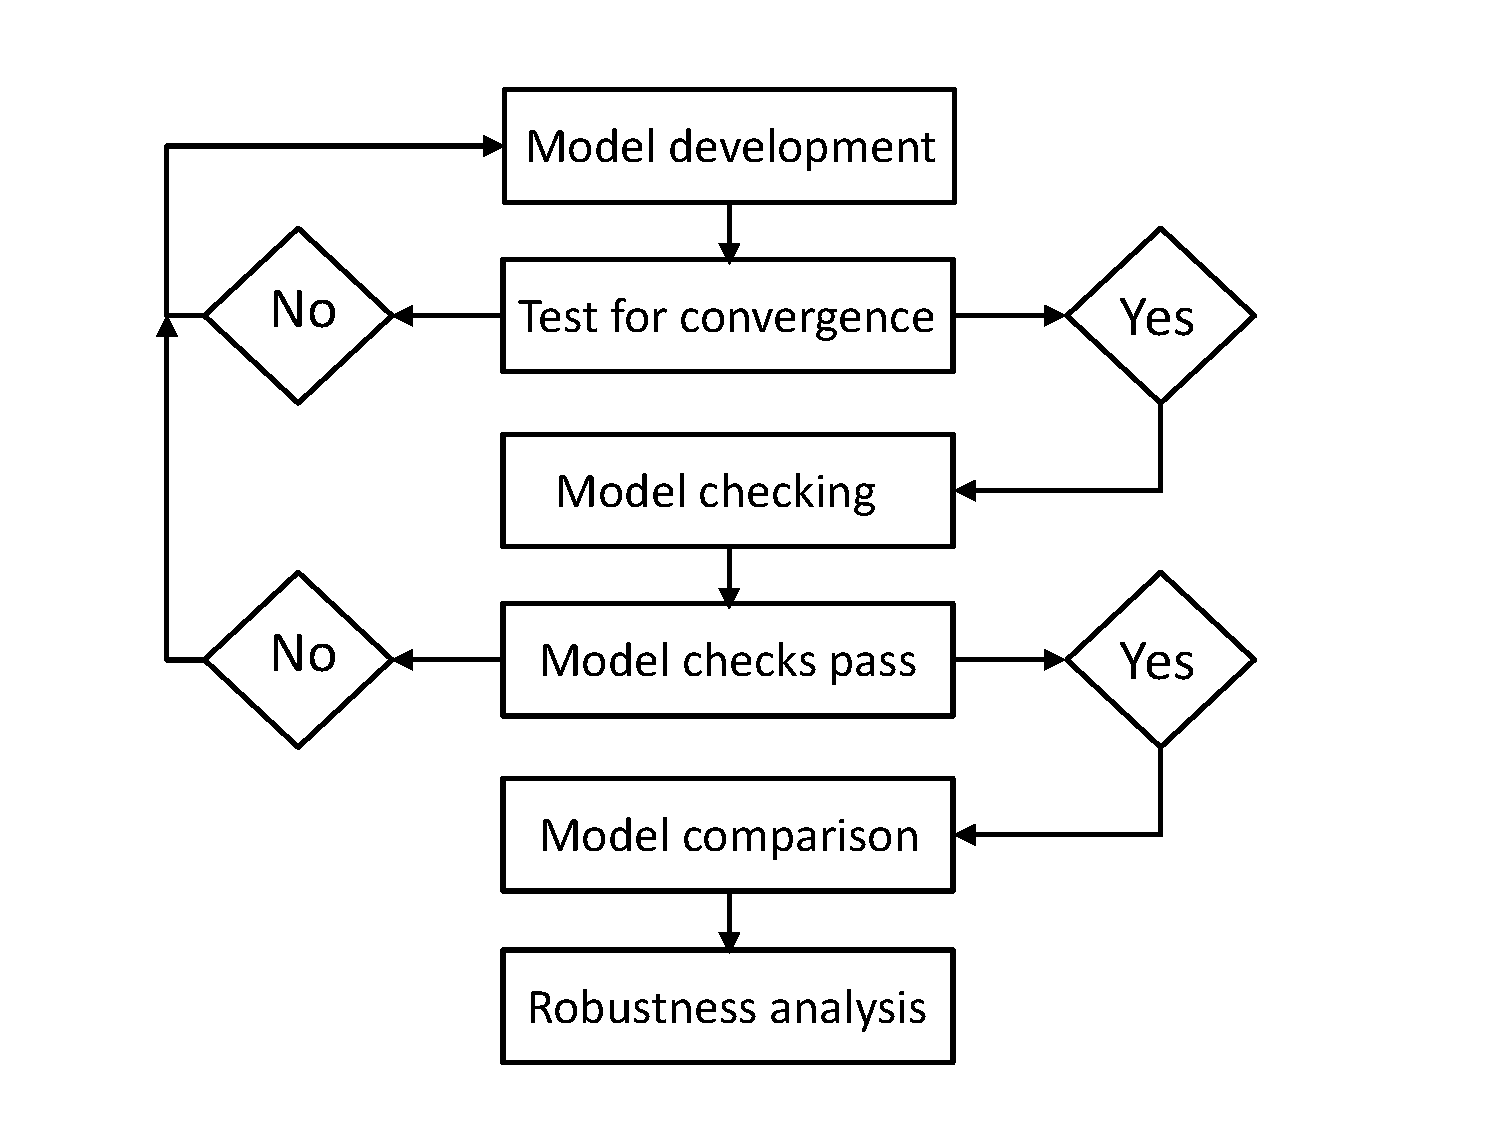
\includegraphics[width=170mm]{Bayesian_modeling_decision_diagram.pdf}
\caption{} \label{fig:decision}
\end{center}
\end{figure*}

\begin{figure*}
\begin{center}
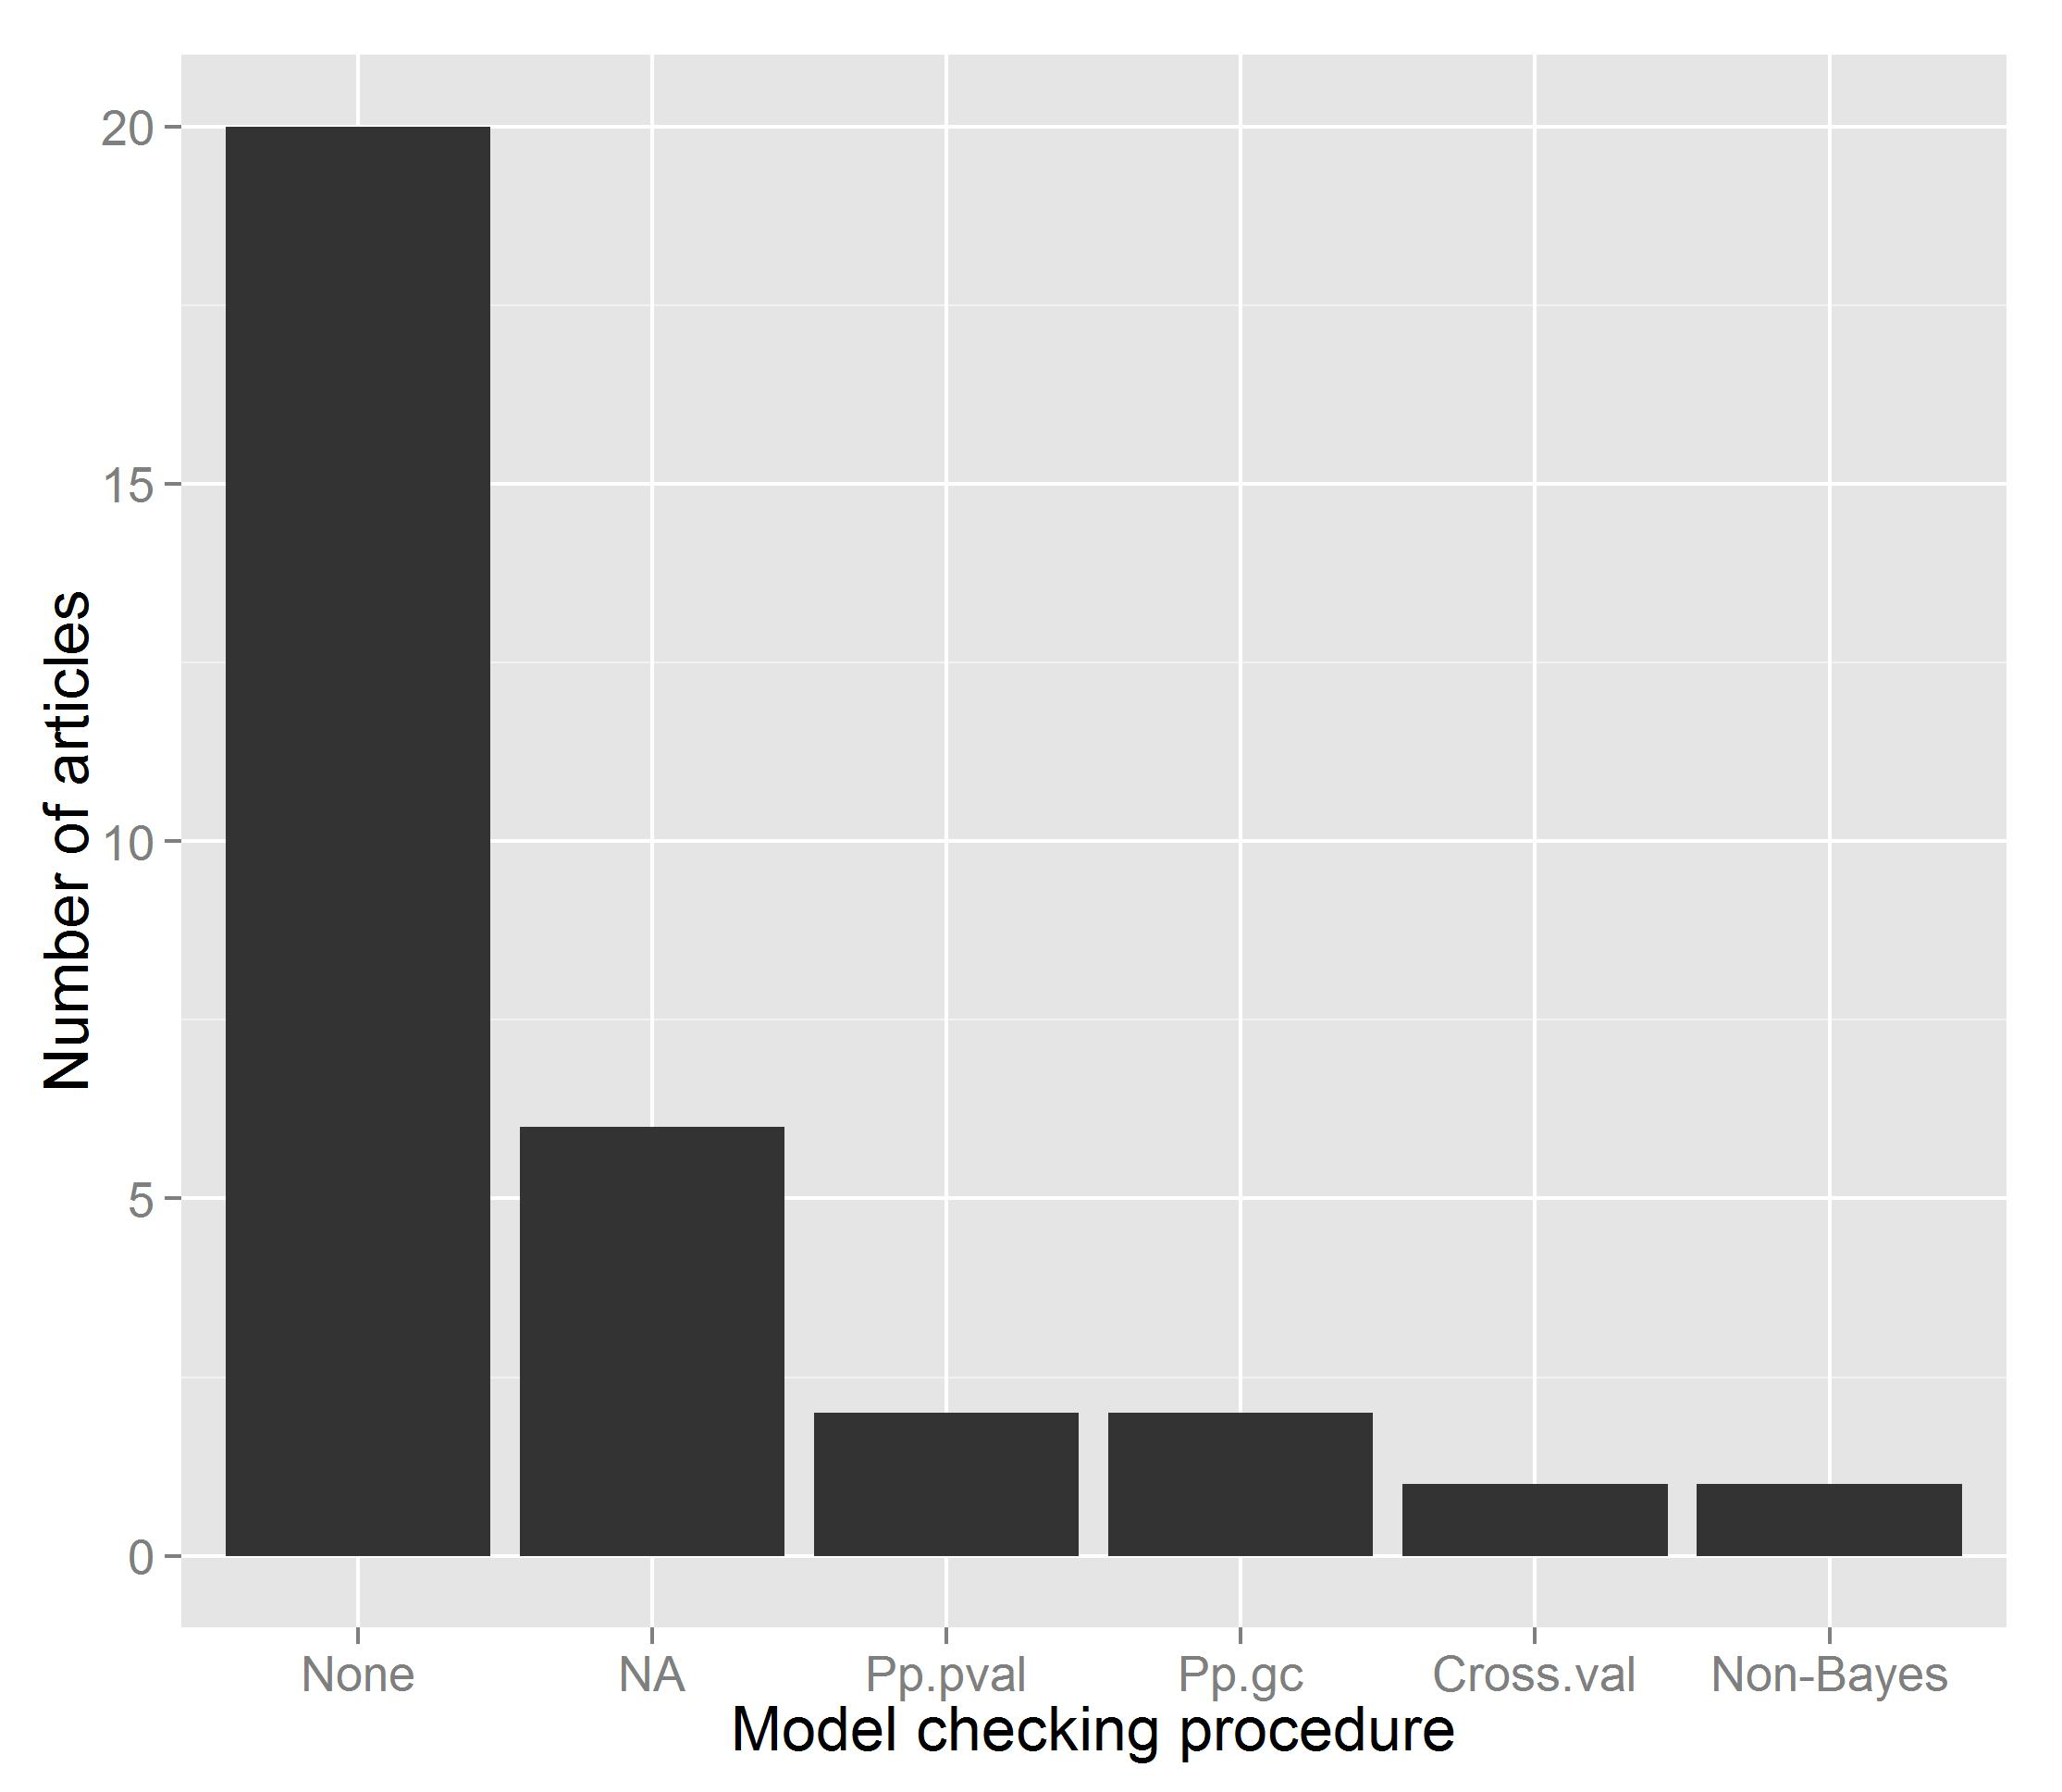
\includegraphics[width=170mm]{WOSsearch.jpeg}
\caption{} \label{fig:WOS}
\end{center}
\end{figure*}

\begin{figure*}
\begin{center}
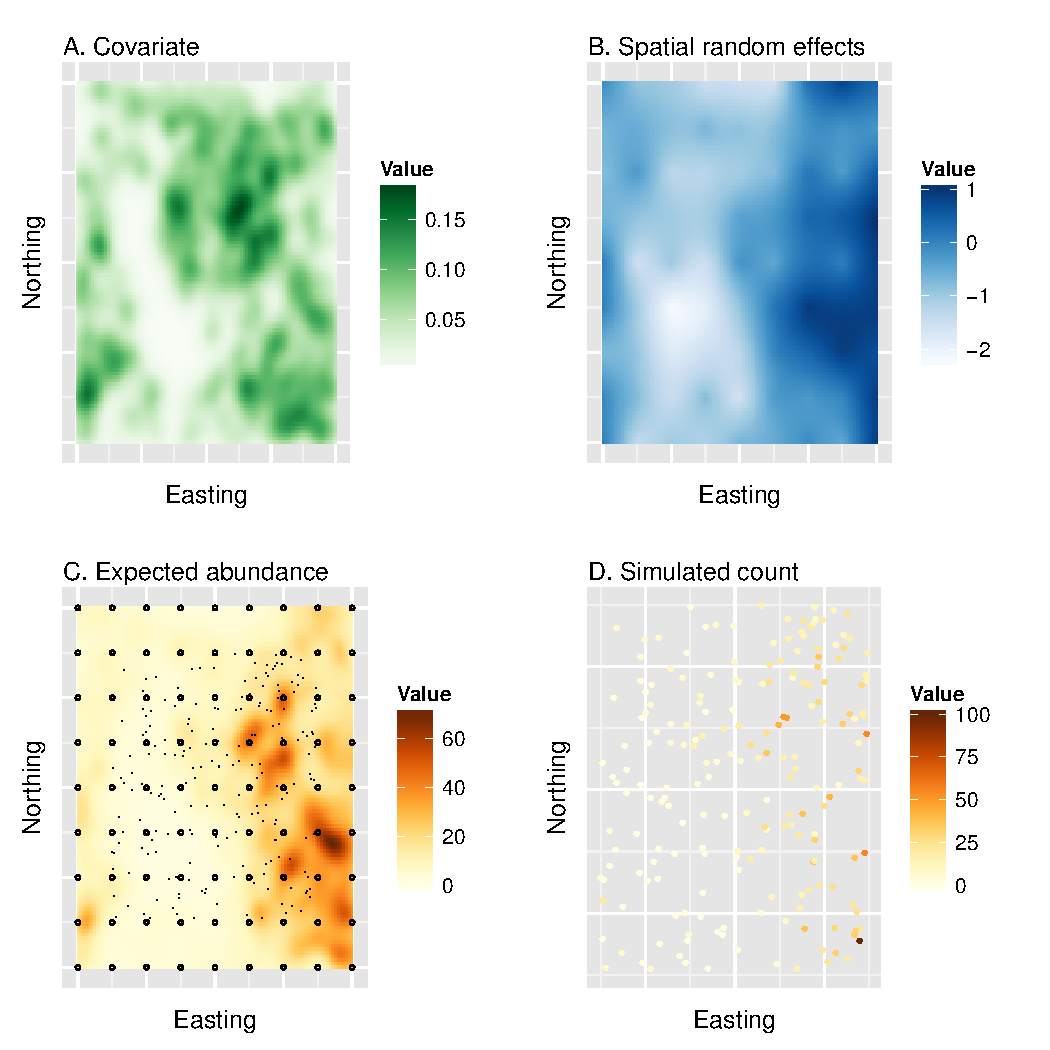
\includegraphics[width=170mm]{sim_count_maps.pdf}
\caption{} \label{fig:sim_maps}
\end{center}
\end{figure*}

\begin{figure*}
\begin{center}
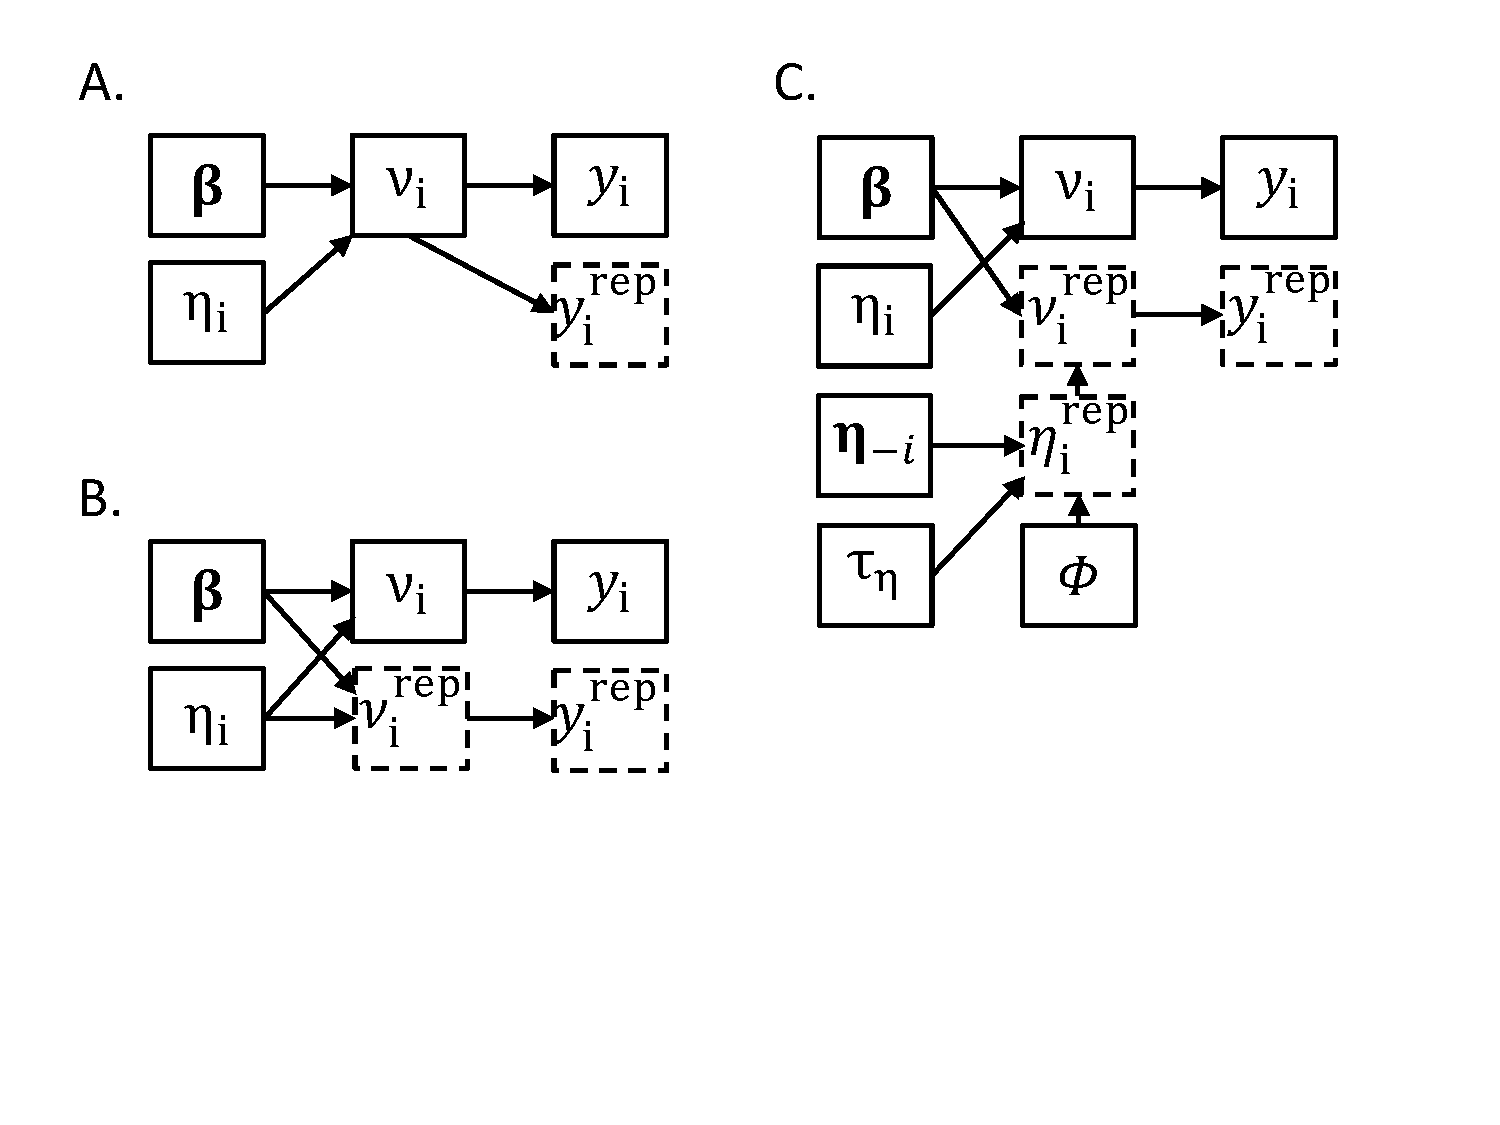
\includegraphics[width=170mm]{posterior_prediction_diagram.pdf}
\caption{} \label{fig:post_pred}
\end{center}
\end{figure*}

\begin{figure*}
\begin{center}
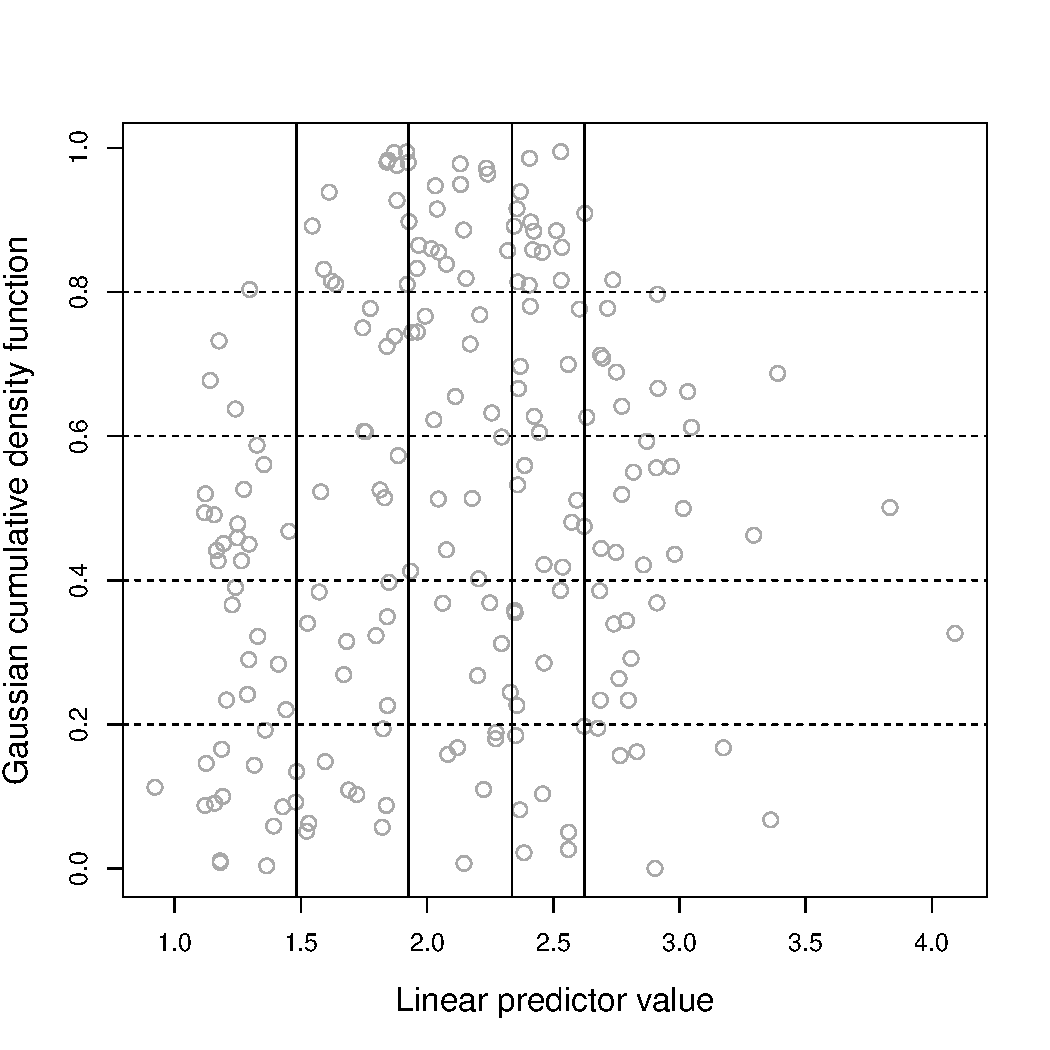
\includegraphics[width=170mm]{pivot_CDF_plot.pdf}
\caption{} \label{fig:pivotCDF}
\end{center}
\end{figure*}

\begin{figure*}
\begin{center}
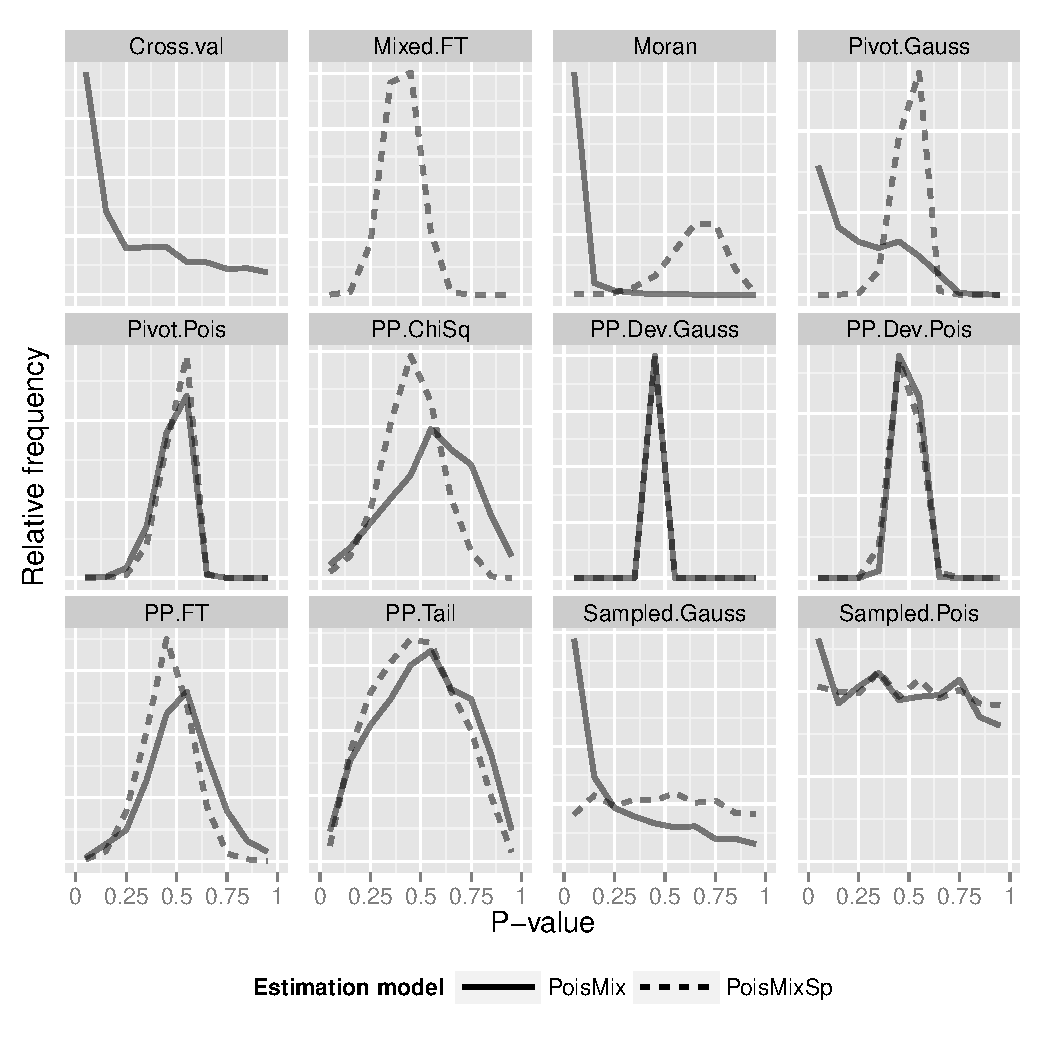
\includegraphics[width=170mm]{SpatRegSimPvals.pdf}
\caption{} \label{fig:SpatReg_pvals}
\end{center}
\end{figure*}

\end{spacing}
\end{document}
